\documentclass[12pt,a4paper]{article}
\usepackage[utf8]{inputenc}
\usepackage[T1]{fontenc}
\usepackage[margin = 0.5in, top = 1in]{geometry}
\usepackage{fancyhdr}
\usepackage{physics}
\usepackage{amssymb}
\usepackage{graphicx}
\usepackage{hyperref}
\usepackage{float}
%\usepackage{subfig}
\usepackage{caption,subcaption}
\usepackage{tikz}
\usetikzlibrary{bayesnet}
\usepackage[doublespacing]{setspace}
\usepackage[toc,page]{appendix}
\restylefloat{table}
\pagestyle{fancy}
\fancyhf{}
\newcommand{\Ti}{Statistical Data Analysis 2}
\newcommand{\Author}{Mateusz Kapusta}
\newcommand{\dane}{\mathcal{D}}
\newcommand{\Title}{Project nr 1}
\title{\huge \bf \Title\\
    \large Statistical Data Analysis 2 
}
\author{Mateusz Kapusta}
\DeclareRobustCommand{\bbone}{\text{\usefont{U}{bbold}{m}{n}1}}
\DeclareMathOperator{\EX}{\mathbb{E}}% expected value
\rhead{\it \Ti}
\lhead{\Author}
\begin{document}
\maketitle
\section{Data exploration}
\hspace{1cm}In the project we will use gene expresion matrix with each with measure of mRNA activity. Each row coresponds to one of the cells while columns represent diffrent
genes. In train set we have $72208$ cells with expresion values for $5000$ genes while test set consists of $18052$ cells also with vales for $5000$ diffrent genes.
Values of mRNA expression are depicted on the figure \ref{histograms}. 
\begin{figure}[H]
    \centering
    \includegraphics[scale=0.7]{src/task1_histogram.png}
    \caption{Histogram representing distribution of data in matrices.}\label{histograms}
\end{figure}
We can see that most values of our data is zero, in fact nearly $91\%$ of our values are zero. 
This fact have biological reason, it means that we observed our cell when it was inactive, in order to
see any expresion special circumscences must occure. We have also most important information about each cell mainly about donor (sex,race etc.) but also information
about batch. There are $12$ unique batches, this is something we need to be carefull later. Each batch number represent unique combination of  patient number and lab id,
there are total $10$ patients that were examiend in $4$ diffrerents labs. There are also $45$ unique cell types.
Data is presented in two versions, raw and preprocessed one.
Raw data is purly discrete while preprocessed data is continuous. Data was propably normalized to 10k counts but not transformed using function log1p. 
Also data wasn't normalized to unit variance what can be easly shown when computing standard deviation of preprocessed data.
What should be mentioned preprocessed data has mean $3.46$ and standard deviation of $1436$, it's more 
then values of raw data for which those two parameters are equal $0.44$ and $34$, also range of raw data is smaller then range of preprocessed one. 
Data does not follow any 
easly described distribution, it's heavly zero inflated and does not follow popular discrete distributions like Poisson distribution.

\section{Simple VAE example}
\hspace{1cm} Variational autoencoder is a type of generativ model using ANN to model propabilistic distribution of data. Lets consider Bayesian graphical 
model as on the figure \ref{VAE}.
\begin{figure}[H]
    \centering
    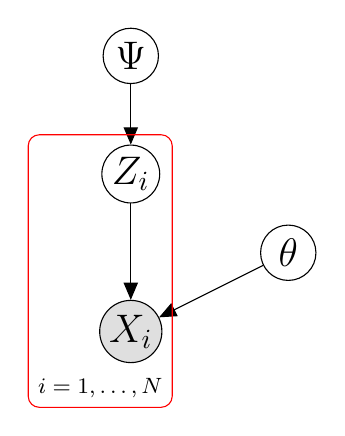
\begin{tikzpicture}
        \node[latent] (psi) at (0,1.5) {\Large $\Psi$};
        \node[latent] (z) at (0,0) {\Large $Z_i$};
        \node[obs] (x)  at (0,-2) {\Large $X_i$};
        \node[latent] (theta) at (2,-1) {\Large $\theta$};
        \path[draw,->] (z) edge (x);
        \path[draw,->] (psi) edge(z);
        \path[draw,->] (theta) edge (x);
        \plate [color=red] {part1}  {(z)(x)} {$i=1,\ldots,N$};
    \end{tikzpicture}
    \caption{Bayesian net model for variational autoencoder}
    \label{VAE}
    \centering
\end{figure}
In our basic case we have latent space $\vb{Z}$ which have prior $\Psi$. We assume gaussian prior $\vb{\Psi} \sim \mathcal{N}(0,\vb{1})$,
bold font stands for n-th dimensional shape. We denote $\theta$ parameters of the decoder which computes parameters of probability of $\vb{X}$.
In case of VAE stricly speeking we are modeling $P(\vb{X}|\vb{Z},\theta)$ using suitable neural netowork. 
We also want to aproximate posterior distribution $p_{\theta,\psi}(\vb{Z}|\vb{X})\approx q_\varphi(\vb{X}|\vb{Z})$ using other neral network called encoder 
denoted by $\varphi$. We will select such models that
\begin{align}
    q_\varphi(\vb{Z}|\vb{X})\sim \mathcal{N}(f_\varphi(\vb{X}),h_\varphi(\vb{X}))
\end{align}
where $f$, $h$ and $g$ functions modeled by neural networks. We constrain posterior probability to normal distribution with diagonal covariance matrix.
On labolatory we used two reconstruction losses: MSE and binary crossentropy. Both losses have some background in propabilistic approach. Lets write loss function
(-ELBO) for our case:
\begin{equation}
    \mathcal{L}(\mathcal{D})=-\EX_{q_\varphi}\log{ P_\theta(\vb{X}|\vb{Z})}+D_{KL}(q_\phi(\vb{Z}|\vb{X})|\mathcal{N}(0,\vb{1}))
\end{equation}. We want to assume, that the expression of each gene is independent from each other so 
$P(X_1,\ldots,X_n)=P(X_1)\cdot\ldots \cdot P(X_n)$.
Moreover we want neural network to produce $n$ sets of parameters $\mu_i$ that will be parametrizing those distribution. If we assume that our 
distribution is 
\begin{equation}
    p(X_i|\mu_i)=\mathcal{N}(\mu_i,\sigma)
\end{equation}
where $\sigma$ is simple hyperparameter. We then have 
\begin{equation}
    \log{P(\vb{X}|\vb{Z})}=\sum \frac{(\mu_i(\vb{Z})-X_i)^2}{2\sigma^2}+C.
\end{equation} Hence we can see that when we assume gaussian probability model our approach will be equal to minimalizing MSE reconstruction loss if 
$\sigma=\frac{1}{\sqrt{2}}$. $\sigma$ is hyperparameter and hence can be chosen freely allowing us to control relative importance of reconstruction loss
and KL divergence. In our decoder $\sigma=1$ will be used as default value of standard deviation.
\subsection{Implementation}
In order to implement variational autoencoder Pyro package was used. In this particular VAE preprocessed data was used as it have continuous distribution so 
is more sutable to model with gaussian distribution then raw thata that takes discrete values only. Each layer of neural network consist of dense layer followed
by batch normalization and ReLu activation layer with dropout $p=5\%$. This setup prevents VAE from overfitting and also allows to deal with numerical
problems with variance. Decoder and encoder consisted of 2 hidden layers with $500$ and $200$ hidden neurons (in different order). Encoder was also supplied with
normalization layer which preprocessed data to have zero mean and unit variance. As encoder need to output standard deviation of gaussian distribution one of the 
two outputs was then passed through ReLU function. Decoder output was also passed through ReLU function
as we deal with positive data only. VAE was trained using batch size equal to $128$ with learning rate $3\cdot10^{-3}$ for $600$ epoches. Learing rate was multiplied by factor of $0.6$ after $100$ epoches allowing
to achive better accuracy over time. In order to find out optimal hyperparameters such as latent size  small grid search was performed using 5 latent
space dimensions.Values of  $-ELBO$ loss on test set  after $200$, $400$ and $600$ epoches is reported together with explained variance ratio for latent space by three first components
of PCA (denoted as $\sigma_{PCA_i}$) in table \ref{table:gauss}. 
\begin{center}
    \begin{table}[H]
    \begin{tabular}{ |c| c| c |c |c |c| c| }
    \hline \hline
     Latent space size & $-ELBO_{200}$ [$10^9$] & $-ELBO_{400}$ [$10^9$] & $-ELBO_{600}$ [$10^9$] & $\sigma_{PCA_1}$ &$\sigma_{PCA_2}$ &$\sigma_{PCA_3}$ \\    
    \hline \hline
    $50$ & 9.532 &8.564 &8.243& 0.682 & 0.160 & 0.088 \\ 
    \hline
    $70$ & 9.526 &8.490 & 8.246& 0.621 & 0.261 & 0.072 \\
    \hline
    $100$ & 9.508 & 8.568& 8.231 & 0.761 & 0.132 &0.072\\
    \hline
    $120$ & 9.643 & 8.634& 8.252 & 0.809 & 0.122 &0.048\\
    \hline
    $150$ & 9.629 & 8.531 & 8.160 & 0.535 & 0.380 &0.04\\
    \hline \hline
\end{tabular}
\caption{ELBO values for test set together with ratio of variance explained with PCA components}\label{table:gauss}
\end{table}
\end{center}
We can see, that in all cases 95\% of variance is achived when we use just using $3$ PCA components (except for latent size $50$ when we need $4$ components). 
We can infer from data, that latent space does not affect values of ELBO so much. What we need to adress are huge values of our loss function. This output is 
not proportional to MSE loss as we also have rather big constant resulting from $\log{2\pi \sigma^2}$ which is also included. Morover we assumed that our $\sigma$
is just equal to 1, assumption which looks rather wrong when we come back to parameters of our data, standard deviation of test set is more then thousend.
More serious approach should deal with this problem and come with more realistic value of $\sigma$. After PCA fit each test data was mapped onto 
first two components of PCA and then colored using cell type, relevant plots are presented on figure \ref{fig:1}.

\begin{figure}[H] % "[t!]" placement specifier just for this example
    \begin{subfigure}{0.48\textwidth}
    \includegraphics[width=\textwidth]{src/gaussian_pca_50.png}
    \caption{Latent size $50$}
    \end{subfigure}\hspace*{\fill}
    \begin{subfigure}{0.48\textwidth}
    \includegraphics[width=\textwidth]{src/gaussian_pca_70.png}
    \caption{Latent size $70$}
    \end{subfigure}
    
    \medskip
    \begin{subfigure}{0.48\textwidth}
    \includegraphics[width=\textwidth]{src/gaussian_pca_100.png}
    \caption{Latent size $100$} 
    \end{subfigure}\hspace*{\fill}
    \begin{subfigure}{0.48\textwidth}
    \includegraphics[width=\textwidth]{src/gaussian_pca_120.png}
    \caption{Latent size $120$}
    \end{subfigure}
    
    \medskip
    \begin{subfigure}{0.48\textwidth}
    \includegraphics[width=\textwidth]{src/gaussian_pca_150.png}
    \caption{Latent size $150$}
    \end{subfigure}\hspace*{\fill}
    
    \caption{PCA mapping of test set for Gausian decoder.} \label{fig:1}
    \end{figure}


From all of the models it was decided to choose model with laten space size $100$ due to the low ELBO values and high ratio of explained variance. 
Learing curve of the model is presented on the figure \ref{fig:vanila_train}.
\begin{figure}[H]
    \begin{center}
        \includegraphics[scale=0.4]{src/vanila_VAE_training_100.png}
    \end{center}
    \caption{Learing curve for Gaussian VAE}
    \label{fig:vanila_train}
\end{figure}
We can see, that hyperparameters $\sigma$ which we are using lead to reconstruction loss dominating ELBO. This have rather bad efffect on our VAE,
due to this behaviour KL loss part is rising making our VAE more similar to normal autoencoder. We can also clearly see, that test loss is circa 3 times 
higher then train error. This behaviour is very suspicious as it indicates that propably test data was preprocessed using different values then train data. 
PCA was trained od train data and then subsample of test data was mapped onto two first axis of PCA ($2500$ subsamples). 
Resulting plot is presented on the figure \ref{fig:pca_gauss}.
\begin{figure}[H]
    \begin{center}
        \includegraphics[scale=1]{src/gaussian_pca_100.png}
    \end{center}
    \caption{Mapping of test data onto first two components of PCA trained on train set.}
    \label{fig:pca_gauss}
\end{figure}
\section{Negative Binomial VAE}
In order to model our data more accurate we want to model not preprocessed data but raw one. One of the distributions which can be used to model discrete data
is poisson distribution. We can clearly see, that mean is not equall to variance of our distribution which is true for poisson distributed data. 
Instead of Poisson distribution one can use zero inflated one or negative binomial distribution. We will use second option which is parametrised by 2 parameters,
number of total counts $r$ and probability $p$. We model bouth values using neural network using setup similar to encoder, last hidden layer is connected to 
2 output layers, one for parameter $t$ and second for parameter $p$. Log probability of our distribution is equal to
\begin{equation}
    \log{P(x=k|r_i,p_i)}=\log{\left({k+r-1\choose k}(1-p)^k p^r\right)}
\end{equation}.
\subsection{Implementation}
This type of VAE was implemented using very similar setup as in previous subtask with main differences in decoder. Instead of big decoder with two
hidden layers with $200$ and $500$ neurons setup was swiched to one with one hidden layer with $200$ neurons. Hidden layer
was connected to $2$ outputs layers modeling $r$ and logits of $p$ parameter of Negative Binomial distribution. $r$ parameter was forced to be positve using
ReLU function. Encoder was adopted from Gaussian VAE, only diffrence was GELU activation function which was used instead of ReLU (there was also normalizing layer!).
Also training process was similar as in the case of Gaussian VAE, only value  of learning rate was 3 times smaller at the start.
As declared VAE was trained using raw data instead of preprocessed one. In order to find optimal size of latent space search similar to one with gaussian decoder 
was performed and results can be found in table below.
\begin{center}
\begin{table}[H]
    \begin{tabular}{ |c| c| c |c |c |c| c| }
    \hline \hline
     Latent space size & $-ELBO_{200}$ & $-ELBO_{400}$ & $-ELBO_{600}$ & $\sigma_{PCA_1}$ &$\sigma_{PCA_2}$ &$\sigma_{PCA_3}$ \\    
    \hline \hline
    $70$ & 1425 &1423 &1421& 0.802& 0.078 & 0.027 \\ 
    \hline
    $100$ & 1438 &1434 & 1432& 0.768 & 0.093 & 0.034 \\
    \hline
    $120$ & 1429 & 1424& 1423 & 0.807 & 0.065 &0.027\\
    \hline \hline
\end{tabular}
\caption{ELBO and PCA variance ration values for  Negative Binomial VAE.}
\end{table}
\end{center}
After considorations it was decided to use latent size $100$. 
Learning curve for training is presented at figure \ref{fig:binomial_train}.
\begin{figure}[H]
    \begin{center}
        \includegraphics[scale=0.4]{src/custom_vae_training_100.png}
    \end{center}
    \caption{Learing curve for Nagative Binomial VAE.}
    \label{fig:binomial_train}
\end{figure}
Few things can be noticed as we can clearly see, that both training and test data give similar error which solves problem that we encountered in previous 
section. KL loss is very stable and is decreasing during training process contrary to Gaussian VAE. Also values of $-ELBO$ are much smaller which tells us 
that our model is better description of reality. We can also compare PCA fits of latent spaces for both decoders which can we see on \ref{fig:compare_pca}.
\begin{figure}[H]
    \begin{center}
        \includegraphics{src/compare.png}
    \end{center}
    \caption{Comparsion of PCA fits.}
    \label{fig:compare_pca}
\end{figure}
PCA fit on our Binomial VAE is rather good, we need $5$ or $6$ components to recover $95\%$ of variance. There are many diffrences between those
two plots, second one seem to be much more concentrated.
Lets also color our data by batch information.
Relevant plot is presented on figure \ref{fig:compare_batch}
\begin{figure}[H]
    \begin{center}
        \includegraphics{src/compare_ext.png}
    \end{center}
    \caption{Comparsion of PCA fits with batch information.}
    \label{fig:compare_batch}
\end{figure}
\section{Batch adjusted VAE} 
Let's consider model presented on figure \ref{fig:VAE_batch}.
\begin{figure}[H]
    \centering
    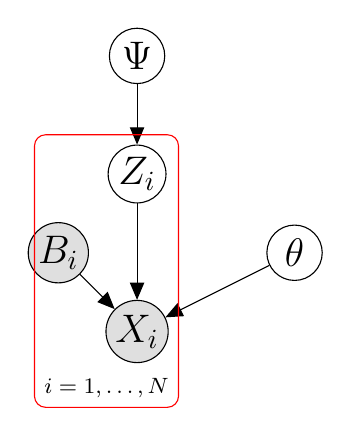
\begin{tikzpicture}
        \node[latent] (psi) at (0,1.5) {\Large $\Psi$};
        \node[latent] (z) at (0,0) {\Large $Z_i$};
        \node[obs] (b) at (-1,-1) {\Large $B_i$};
        \node[obs] (x)  at (0,-2) {\Large $X_i$};
        \node[latent] (theta) at (2,-1) {\Large $\theta$};
        \path[draw,->] (z) edge (x);
        \path[draw,->] (psi) edge(z);
        \path[draw,->] (theta) edge (x);
        \path[draw,->] (b) edge (x);
        \plate [color=red] {part1}  {(z)(x)} {$i=1,\ldots,N$};
    \end{tikzpicture}
    \caption{Bayesian net model for batch adjusted variational autoencoder}
    \label{fig:VAE_batch}
    \centering
\end{figure} Our VAE have additional dependence on varible $B_i$ which represents batch observation. In practice we contancate tensor of one-hot encoded batch
labs with latent space vector and pass it through decoder in order to obtain parameters of our distribution. Here we will use also negative binomial distribution 
as it's working well with our raw data. 
\subsection{Implementataion}
In order to include batch id in our data we one-hot encode vector of lab asignments ant then contancat it with latent vector before passing it through decoder.
Setup from previus task was adopted with all parameters except that decoder at the entry layers has increased width by $12$. Model was also trained using raw 
data for $600$ epoches. Size of latent space was also found using small grid search, values for different batch sizes are presented in  table \ref{table_batch}.
\begin{center}
\begin{table}[H]
    \begin{tabular}{ |c| c| c |c |c |c| c| }
    \hline \hline
     Latent space size & $-ELBO_{200}$ & $-ELBO_{400}$ & $-ELBO_{600}$ & $\sigma_{PCA_1}$ &$\sigma_{PCA_2}$ &$\sigma_{PCA_3}$ \\    
    \hline \hline
    $70$ & 1413 &1409& 1409& 0.898 &0.047 & 0.022 \\ 
    \hline
    $100$ & 1407 &1404 & 1403& 0.865 & 0.065 & 0.014 \\
    \hline
    $120$ & 1415 & 1411& 1410 & 0.859 & 0.082 &0.017\\
    \hline \hline
\end{tabular}
\caption{ELBO and PCA variance ration values for batch adjusted VAE.}\label{table_batch}
\end{table}
\end{center}
It can be easly seen, that latent size $100$ is best and in each case $3$ pca components capture $95\%$ of variance. PCA plot of 
Learing curve is shown on the figure \ref{fig:batch_train}.
\begin{figure}[H]
    \begin{center}
    \includegraphics[scale=0.4]{src/batch_VAE_training_100.png}
    \end{center}
    \caption{Learning curve for batch adjusted VAE.}
    \label{fig:batch_train}
\end{figure}
We can see, that values of $-ELBO$ are much smaller then compared to normal case, we can see that semi-supervised approach is working and batch adjustment 
improves our results. On the figure \ref{fig:pca_batch} we can see PCA decomposition of our latent space.
\begin{figure}[H]
    \begin{center}
    \includegraphics[scale=1]{src/negbinom_batch_pca_100.png}
    \end{center}
    \caption{PCA maping of test data onto PCA for batch adjusted VAE.}
    \label{fig:pca_batch}
\end{figure}
\section{Conclusions}
During project three types of VAE were examiend and it was found, two of them  using Negative Binomial distribution and one using Normal distribution. Each of them
was trained and then evaluated, unfortunatly none of them was able to capture any type of clustering wchich can be related to biological activity.
Negative Binomial distribution performed better then Normal distribution which after combination with batch information was able to yield minimal loss but still
high enough making VAE unsuitable to search for any clustering. 
\end{document}